\documentclass[notitlepage,12pt]{article}
\makeindex
%Gummi|065|=)

\usepackage{url}
\usepackage{bbm}
\usepackage{graphicx}
\usepackage{amsmath}
\usepackage{wrapfig}
\usepackage{float}
\usepackage{enumitem}
\usepackage[linewidth=1pt]{mdframed}
\usepackage{amsthm}
\usepackage[a4paper, total={6.27in, 9.69in}]{geometry}
\usepackage{pdfpages}
\usepackage[toc,page]{appendix}
\usepackage{chngcntr}


\counterwithin{figure}{section}
\counterwithin{equation}{section}

\title{\textbf{Julia ODEInterface Experiments}}
\author{Vishal Sontakke}
\date{}

\begin{document}
\maketitle
\tableofcontents
\newpage
\section{Non-stiff equations}
The problems chosen for our tests are the following:
\subsection{The restricted three body problem (AREN)}
\label{sec:Aren}
We will first look at the restricted three body problem. One considers two bodies of masses $1 - \mu$ and $\mu$ in circular rotation in a plane and a third body of negligible mass moving around in the same plane. The equations are (see e.g., the classical textbook Szebehely 1967):
\begin{equation}
\label{eq:threeBody}
\begin{aligned}
	y_1'' &= y_1 + 2y_2' - \mu'\frac{y_1+\mu}{R_1} -\mu \frac{y_1-\mu'}{R_2},\\
	y_2'' &= y_2 - 2y_1' -\mu' \frac{y_2}{R_1} -\mu \frac{y_2}{R_2},\\
	R_1 &= \left(\left(y_1+\mu\right)^2 + y_2^2\right)^{3/2},
	\ \ R_2 = \left(\left(y_1-\mu'\right)^2 + y_2^2\right)^{3/2},\\
	\mu &= 0.012277471, \ \ \mu' = 1 -\mu .
\end{aligned}
\end{equation}
There exist initial values, for example:
\begin{equation}
\label{eq:3bodyIV}
\begin{aligned}
y_1(0) &= 0.994, \ \ y_1'(0) = 0, \ \ y_2(0) = 0,\\
y_2'(0) &= −2.00158510637908252240537862224,\\
t_{end} &= 17.0652165601579625588917206249,
\end{aligned}
\end{equation}
such that the solution is periodic with period $t_{end}$.
\begin{figure}[H]
\centering
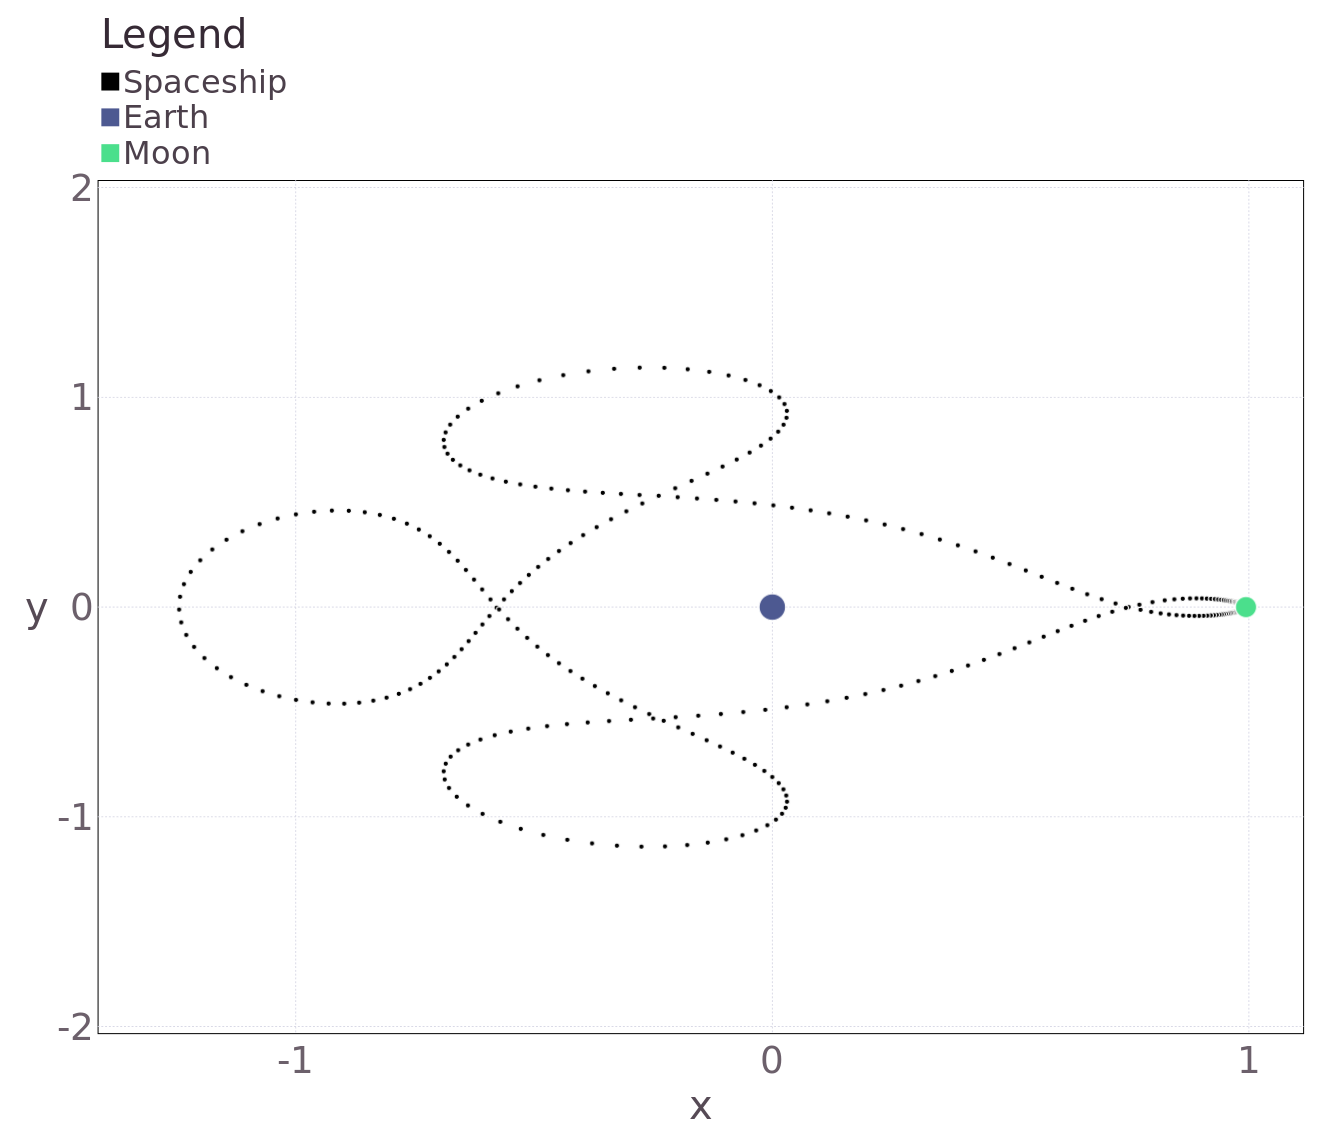
\includegraphics[scale=0.25]{../ImagesAndPDFs/Plots/Arenstorf.png}
\caption{An Arenstorf Orbit computed using Dormand \& Prince}
\label{fig:ArnOrb}
\end{figure}
% section  (end)

\subsection{Movement of hanging rope (ROPE)}
\label{sec:rope}

We look at the movement of a hanging rope of length 1 under gravitation and under the influence of a horizontal force
\begin{equation}
	F_y(t) = \left(\frac{1}{cosh(4t-2.5)}\right)^4
\end{equation} acting at the point $s = 0.75$ as well as a vertical force
\begin{equation}
	F_x(t) = 0.4
\end{equation} acting at the endpoint $s = 1$.\\

If this problem is discretized, then Lagrange theory leads to the following equations for the unknown angles $\theta_k$:
\begin{equation}
\begin{aligned}
\sum _{k=1}^n a_{lk} \ddot{\theta_k} = &-\sum _{k=1}^n b_{lk} \dot{\theta_k}^2 -n\left(n+\frac{1}{2} -l \right)\sin{\theta_l}\\
&-n^2\sin{\theta_l}\cdot F_x(t) + \begin{cases}
               n^2\cos{\theta_l}\cdot F_y(t) &\textnormal{if}\ l\leq 3n/4\\
               0 &\textnormal{if}\ l > 3n/4,
            \end{cases} \ \ \  l = 1,\ldots,n
\end{aligned}
\end{equation}
where
\begin{equation}
	a_{lk} = g_{lk}\cos{(\theta_l -\theta_k)}, \ \ b_{lk} = g_{lk}\sin{(\theta_l -\theta_k)},\ \ g_{lk} = n+\frac{1}{2} - \max{(l,k)}.
\end{equation}
We choose
\begin{equation}
	n=40, \ \ \ \theta_l(0) = \dot{\theta_l}(0) = 0, \ \ \ 0 \leq t \leq 3.723.
\end{equation}

\begin{figure}[H]
\centering
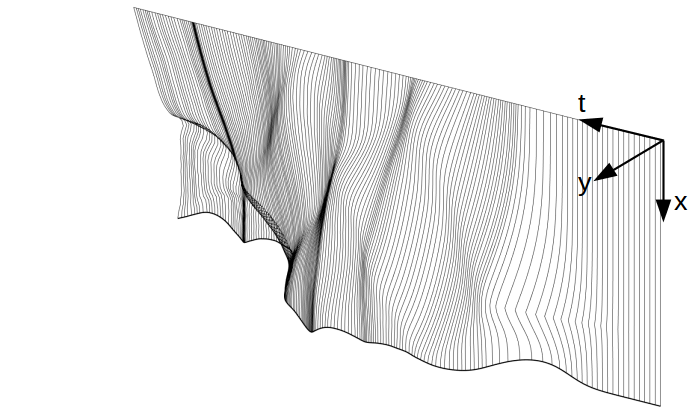
\includegraphics[scale=0.70]{../ImagesAndPDFs/Plots/RopePlot.png}
\caption{Movement of the rope with respect to time}
\label{fig:rope}
\end{figure}

\newpage

\subsection{Code Performance}
\label{sec:codePerfNonStiff}
The three available non-stiff solvers were applied to the above mentioned problems with $Tol = 10^{-3} , Tol =
10^{-3-1/8} , Tol = 10^{-3-2/8}, Tol = 10^{-3-3/8},\ldots$ up to $Tol = 10^{-14}$, then the numerical result at the output points were compared with a "reference solution" using the infinity norm. The "reference solution" is computed using $Tol=1.0\times 10^{-16}$, since quadruple precision is not available on the current hardware (as compared to \cite{nonStiff}). The underlying Fortran codes would have to be tweaked to get quadruple precision using software since Julia can emulate Arbitrary Precision floating point numbers using GNU Multiple Precision Arithmetic Library (GMP) and the GNU MPFR Library.

\subsubsection{AREN}
\label{sub:aren}

\begin{figure}[H]
\centering
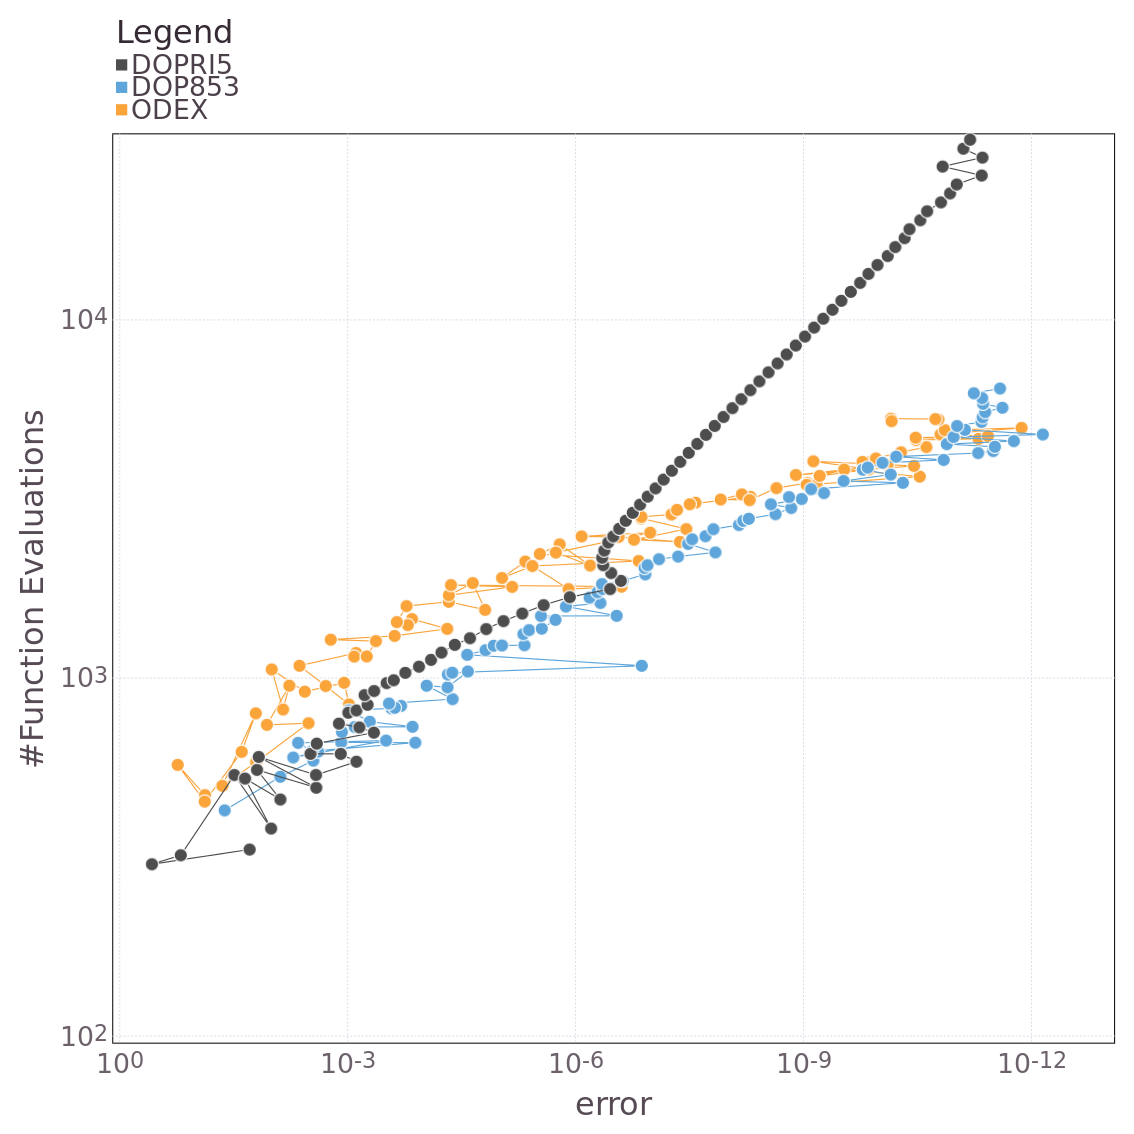
\includegraphics[scale=0.4]{../ImagesAndPDFs/Plots/ArenstorfPrecisionTest.png}
\caption{Precision vs. Number of function evaluations (as computed on Julia using ODEInterface)}
\label{fig:arenJulia}
\end{figure}

\subsubsection{ROPE}
\label{sub:rope}

\begin{figure}[H]
\centering
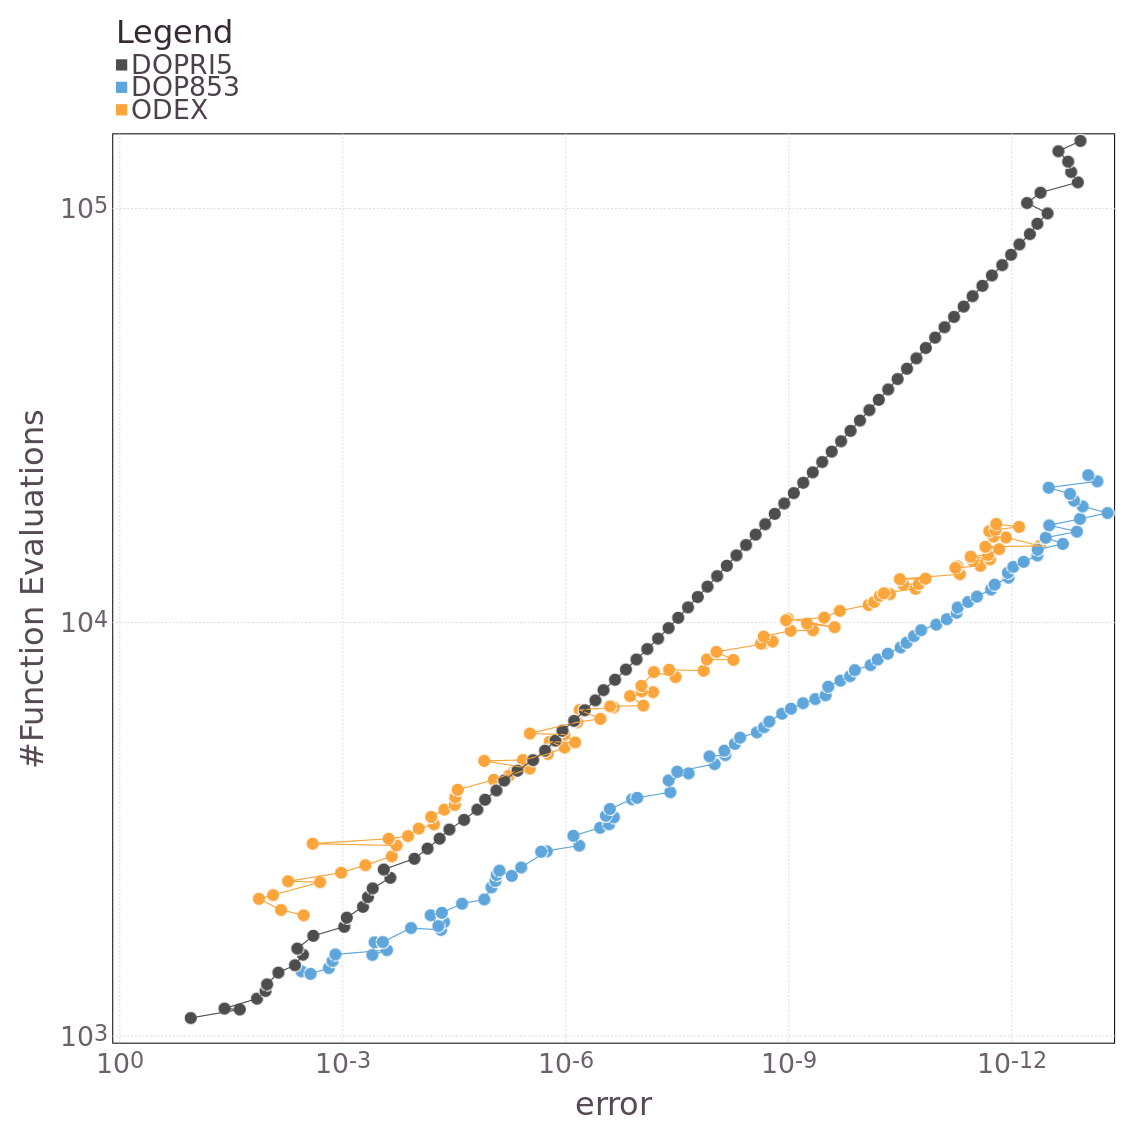
\includegraphics[scale=0.4]{../ImagesAndPDFs/Plots/RopePrecisionTest.png}
\caption{Precision vs. Number of function evaluations (as computed on Julia using ODEInterface)}
\label{fig:ropeJulia}
\end{figure}
% section  (end)

\newpage

\section{Stiff equations}
The problems chosen for our tests are the following:
\label{sec:stiff}

\subsection{Van der Pol oscillator (VDPOL)}
\label{sub:vdpol}
In dynamics, the Van der Pol oscillator is a non-conservative oscillator with non-linear damping. It evolves in time according to the second-order differential equation:
\begin{equation}
\label{vdpolEq}
\frac{d^2x}{dt^2} -\mu \left(1-x^2 \right)\frac{dx}{dt}+x=0,
\end{equation}
where $x$ is the position coordinate-which is a function of time $t$, and $\mu$ is a scalar parameter indicating the non-linearity and the strength of the damping.

The above equation can be converted into a system of first-order differential equations as follows:
\begin{equation}
\begin{aligned}
	x_1' &= x_2\\
	x_2' &= \left(\left(1-x_1^2\right)x_2-x_1\right)/\epsilon, &\epsilon = 10^{-6}\\
\end{aligned}
\end{equation}
We perform a rescaling as follows:
\begin{equation}
\begin{aligned}
\tilde{t} &= t/\mu, &x_1(\tilde{t})&=x(t), &x_2(\tilde{t})=\mu \frac{dx}{dt}(t)\\
\textnormal{and we set}& &\frac{1}{\mu^2} &= \epsilon
\end{aligned}
\end{equation}
This transformation makes the steady state approximation independent of $\mu$.\\ \\
The initial conditions for this problem are:
\begin{equation}
\begin{aligned}
&x_1(0) =2, &x_2(0)&= 0\\
&t_{out} =1,2,3,4,\ldots,11.
\end{aligned}
\end{equation}
The times $t_{out}$ will be the points at which the solution will be taken for comparison.

\begin{figure}[H]
\centering
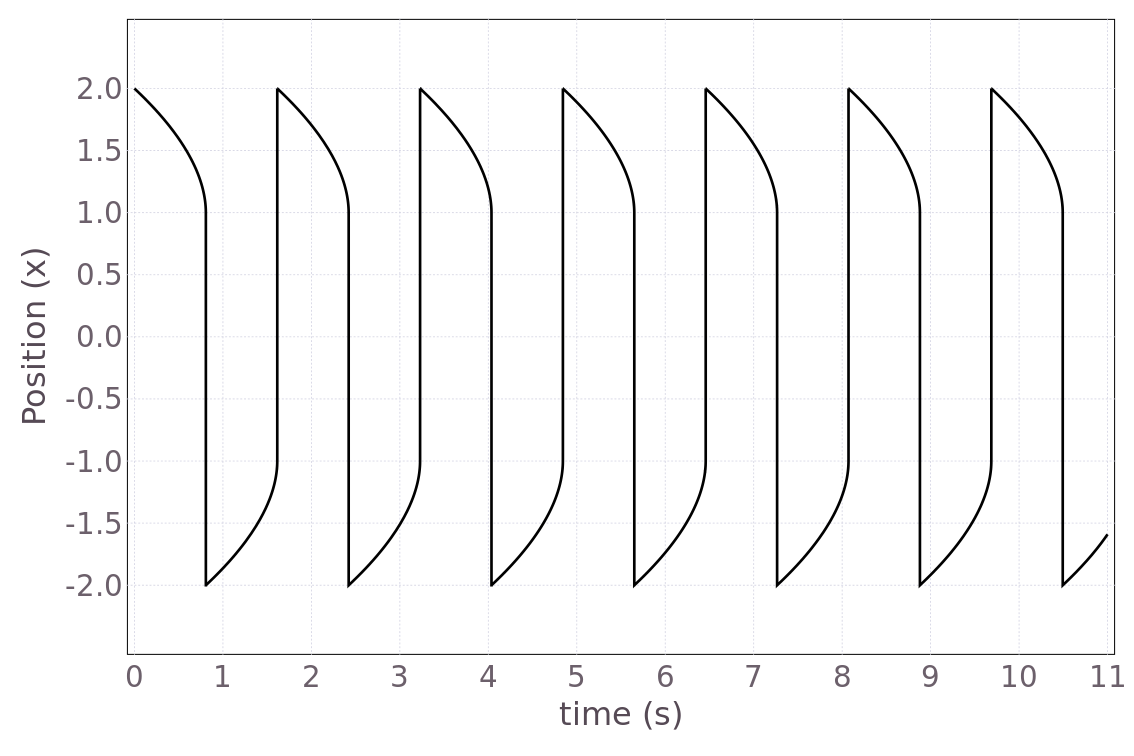
\includegraphics[scale=0.30]{../ImagesAndPDFs/Plots/vdpolPlot.png}
\caption{Solution of equation \eqref{vdpolEq} computed using SEULEX solver}
\label{vdpolPlot}
\end{figure}

% subsection  (end)

\subsection{Robertson Chemical Kinetics (ROBER)}
\label{sub:rober}
The problem describes the kinetics of an auto-catalytic reaction given by Robertson as follows:
\begin{equation}
\label{roberEq}
\begin{aligned}
x_1' &= &-&0.04x_1 &+ &10^4x_2x_3\\
x_2' &= & &0.04x_1 &- &10^4x_2x_3 &-&3\cdot 10^7x_2^2\\
x_3' &= & &        &  &           & &3\cdot 10^7x_2^2.
\end{aligned}
\end{equation}
with initial conditions:
\begin{equation}
x_1(0) = 2, \ \ x_2(0) = 0, \ \ x_3(0) = 0.
\end{equation}
one of the most prominent examples of the "stiff" literature. It was usually treated on the interval $0 \leq t \leq 40$, until Hindmarsh discovered that many codes fail if $t$ becomes very large ($10^{11}$ say). The reason is that whenever the numerical solution of $x_2$ accidentally becomes negative, it then tends to $-\infty$ and the run ends by overflow. We have therefore chosen $t_{out} = 1,10,10^2,10^3,\ldots,10^{11}$.

\begin{figure}[H]
\centering
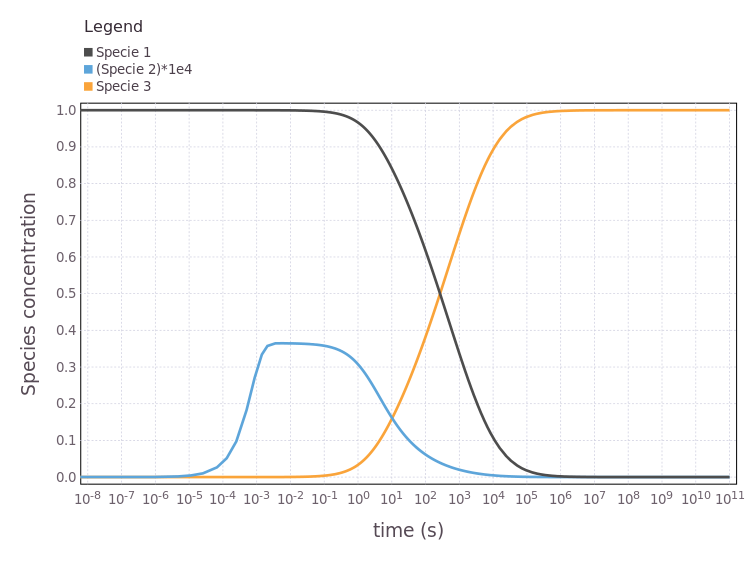
\includegraphics[scale=0.60]{../ImagesAndPDFs/Plots/RoberPlot.png}
\caption{Solution of equation \eqref{roberEq} using SEULEX solver}
\label{fig:roberPlot}
\end{figure}

\newpage
% subsection  (end)

\subsection{Code performance}
\label{sec:codePerfStiff}

The three available stiff solvers were applied to the above mentioned problems with $Tol = 10^{-2} , Tol = 10^{-2-1/4} , Tol = 10^{-2-2/4}, Tol = 10^{-2-3/4},\ldots$ up to $Tol = 10^{-10}$.\\ \\
We set the relative error tolerance to be $RTol=Tol$ and the absolute error tolerance $ATol =10^{-6}\cdot Tol$ for the problem ROBER and $ATol = Tol$ for VDPOL. Then the numerical results were compared with a "reference solution" using the infinity norm (the norm is taken over all components and all output points). The "reference solution" is obtained from \url{http://www.unige.ch/~hairer/testset/testset.html}.

\subsubsection{VDPOL}
\begin{figure}[H]
\centering
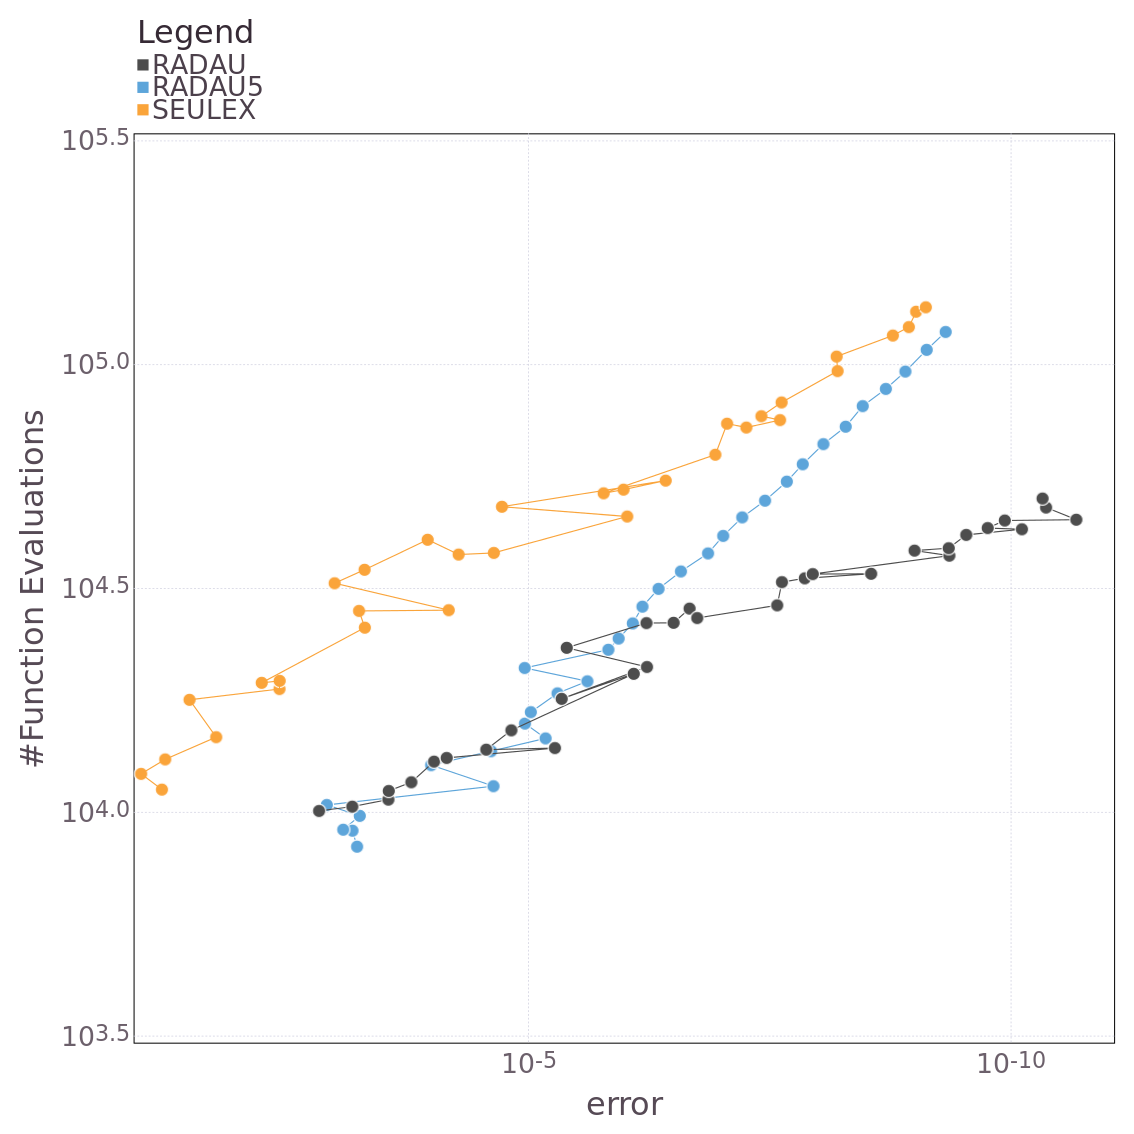
\includegraphics[scale=0.4]{../ImagesAndPDFs/Plots/vdpolPrecisionTest.png}
\caption{Precision vs. Number of function evaluations (as computed on Julia using ODEInterface)}
\label{fig:vdpolJulia}
\end{figure}

\begin{figure}[H]
\centering
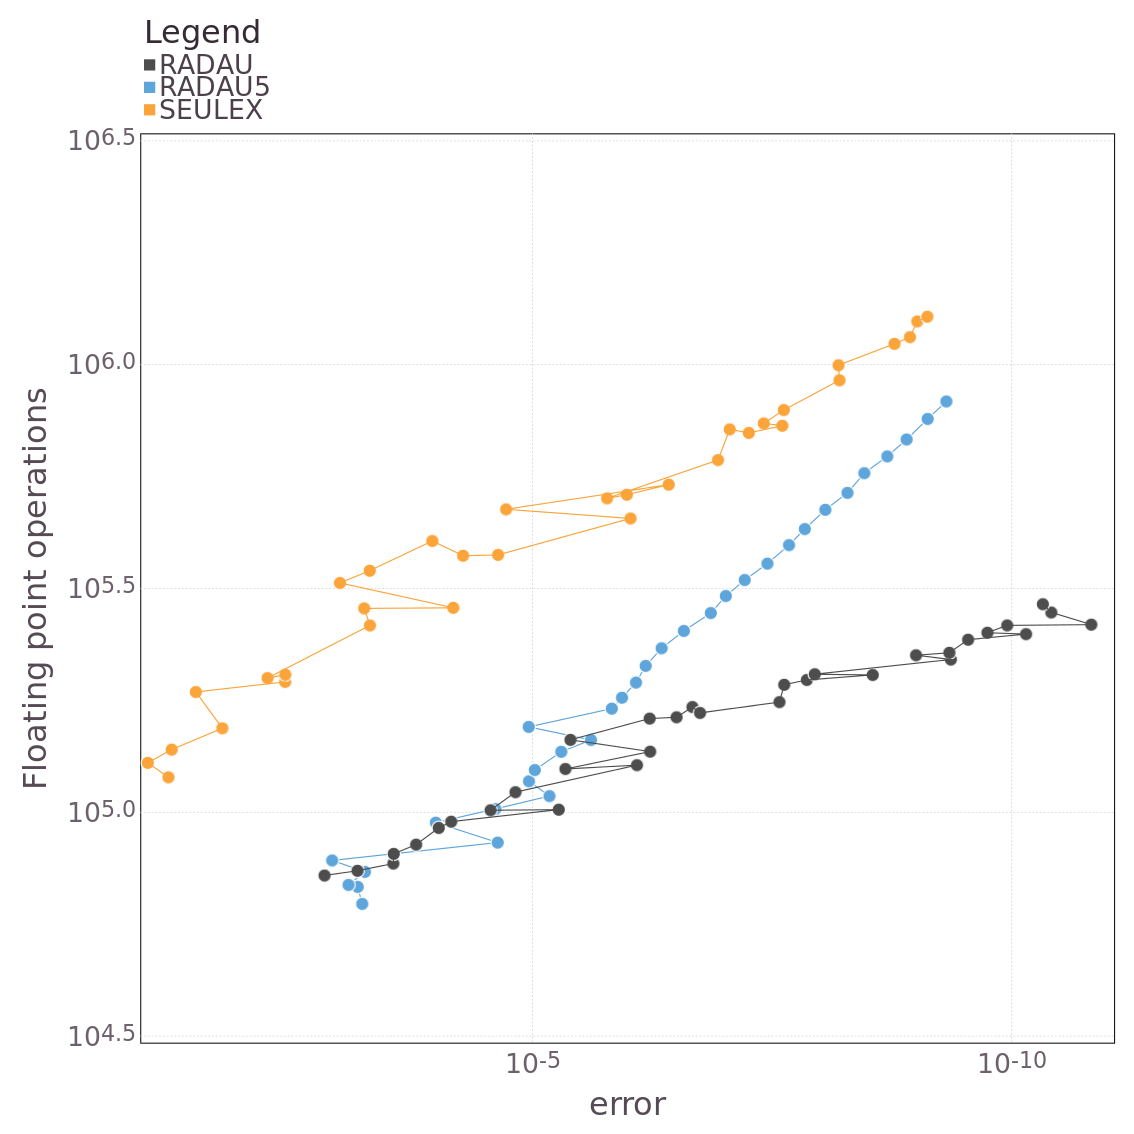
\includegraphics[scale=0.4]{../ImagesAndPDFs/Plots/vdpolPrecisionTestFlops.png}
\caption{Precision vs. Floating point operations (as computed on Julia using ODEInterface)}
\label{fig:vdpolJuliaFlops}
\end{figure}

The following factors were chosen for the various operations:
\begin{itemize}
\item Right-hand side function calls = $5$ flops
\item LU Decomposition = $\lceil \frac{2}{3}\times 8\rceil = 6$ flops
\item Forward or Backward Substitution = $4$ flops
\item Jacobian computation using Automatic Differentiation = $\lceil 1.5*5 \rceil = 8$ flops
\end{itemize}


\subsubsection{ROBER}
\begin{figure}[H]
\centering
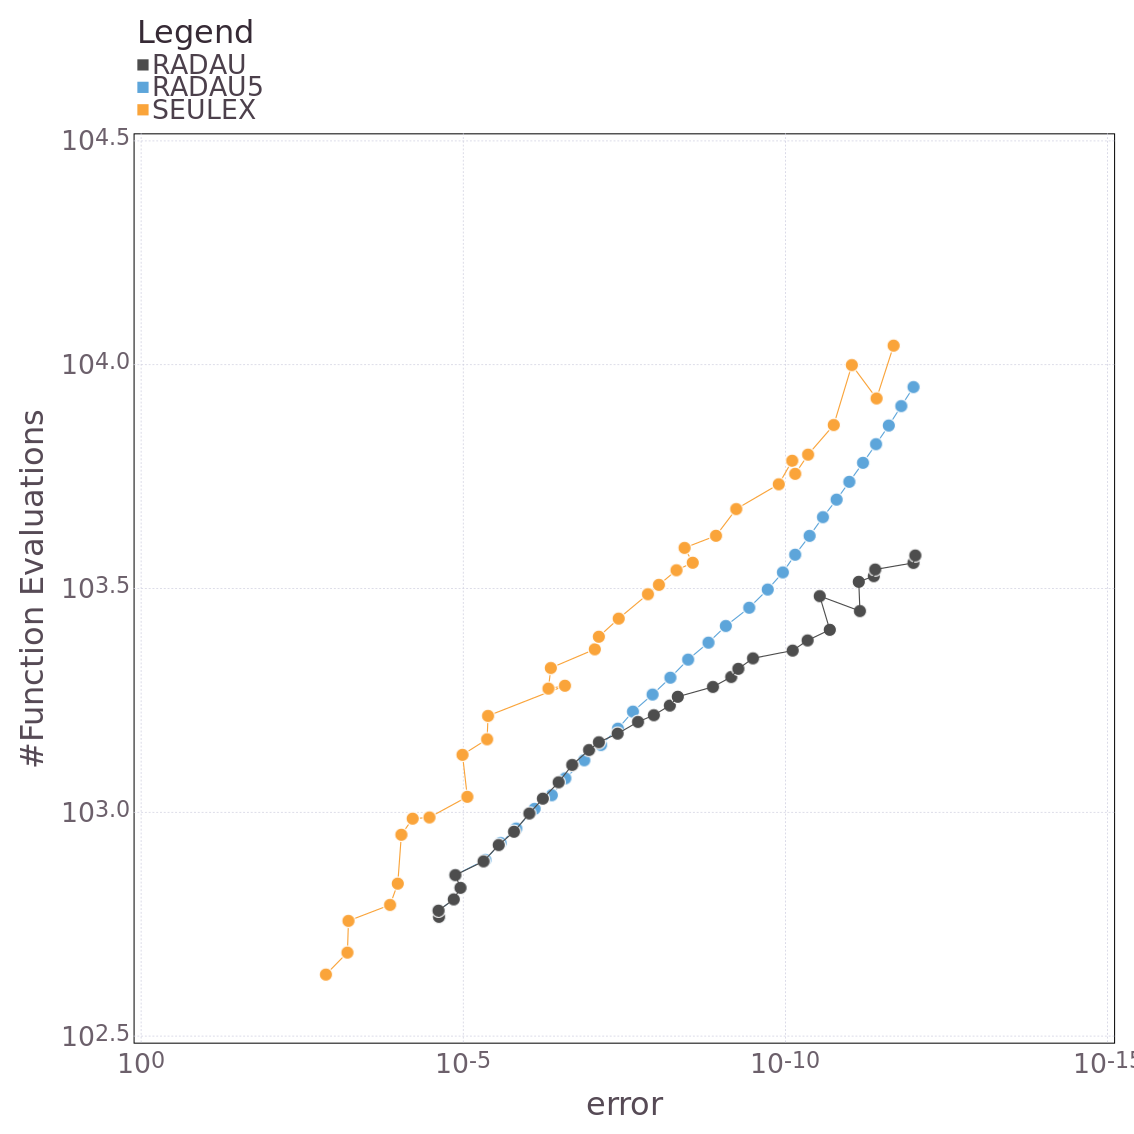
\includegraphics[scale=0.4]{../ImagesAndPDFs/Plots/RoberPrecisionTest.png}
\caption{Precision vs. Number of function evaluations (as computed on Julia using ODEInterface)}
\label{fig:roberJulia}
\end{figure}

\begin{figure}[H]
\centering
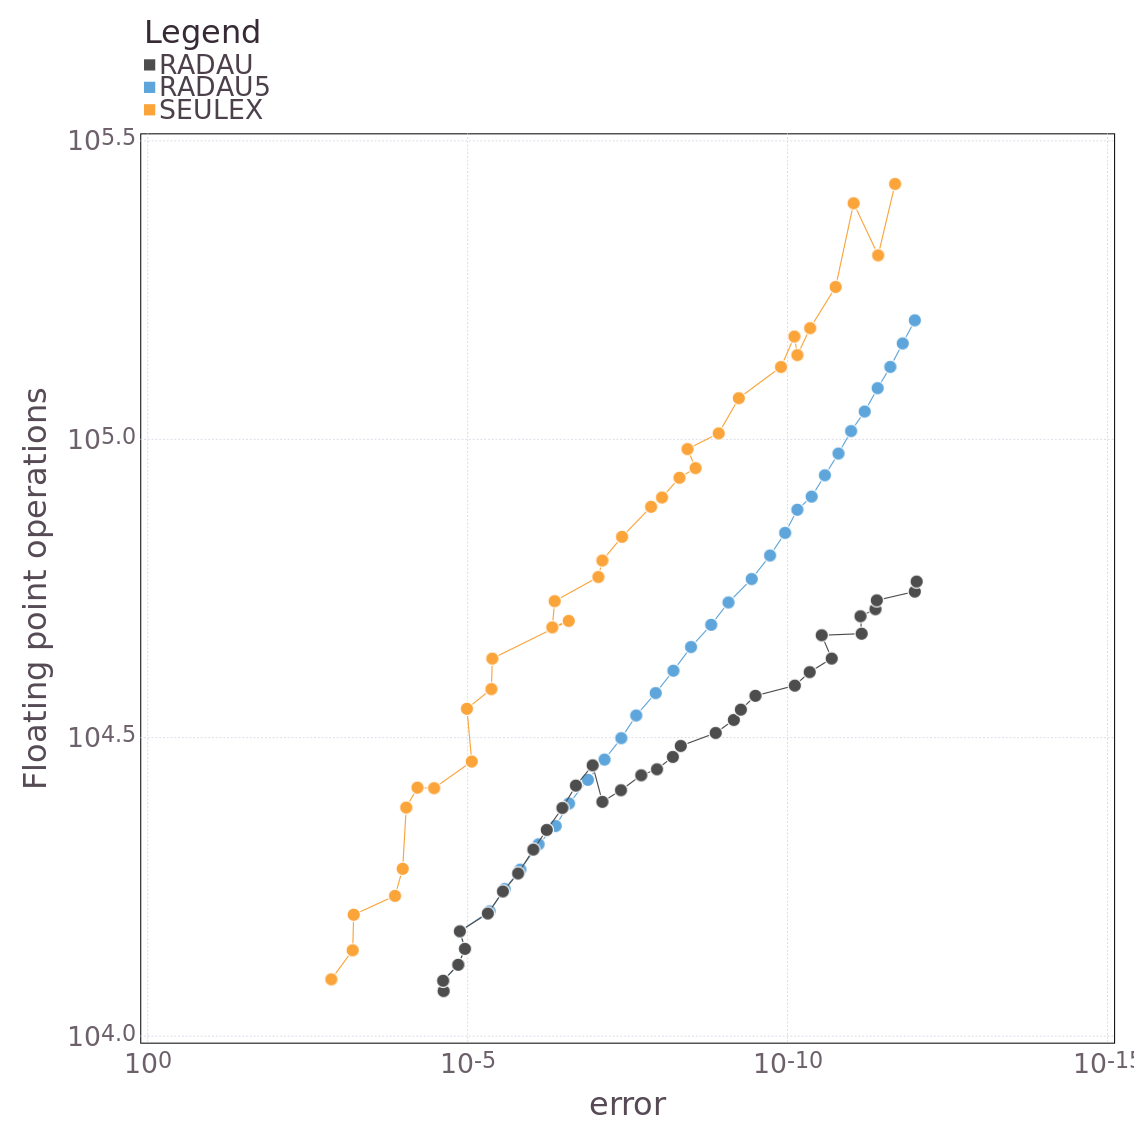
\includegraphics[scale=0.4]{../ImagesAndPDFs/Plots/RoberPrecisionTestFlops.png}
\caption{Precision vs. Floating point operations (as computed on Julia using ODEInterface)}
\label{fig:roberJulia}
\end{figure}

The following factors were chosen for the various operations:\\
\begin{itemize}
\item Right-hand side function calls = $5$ flops
\item LU Decomposition = $\lceil \frac{2}{3}\times 8\rceil = 6$ flops
\item Forward or Backward Substitution = $4$ flops
\item Jacobian computation using Automatic Differentiation = $\lceil 1.5*5 \rceil = 8$ flops
\end{itemize}

% subsection  (end)

% section  (end)

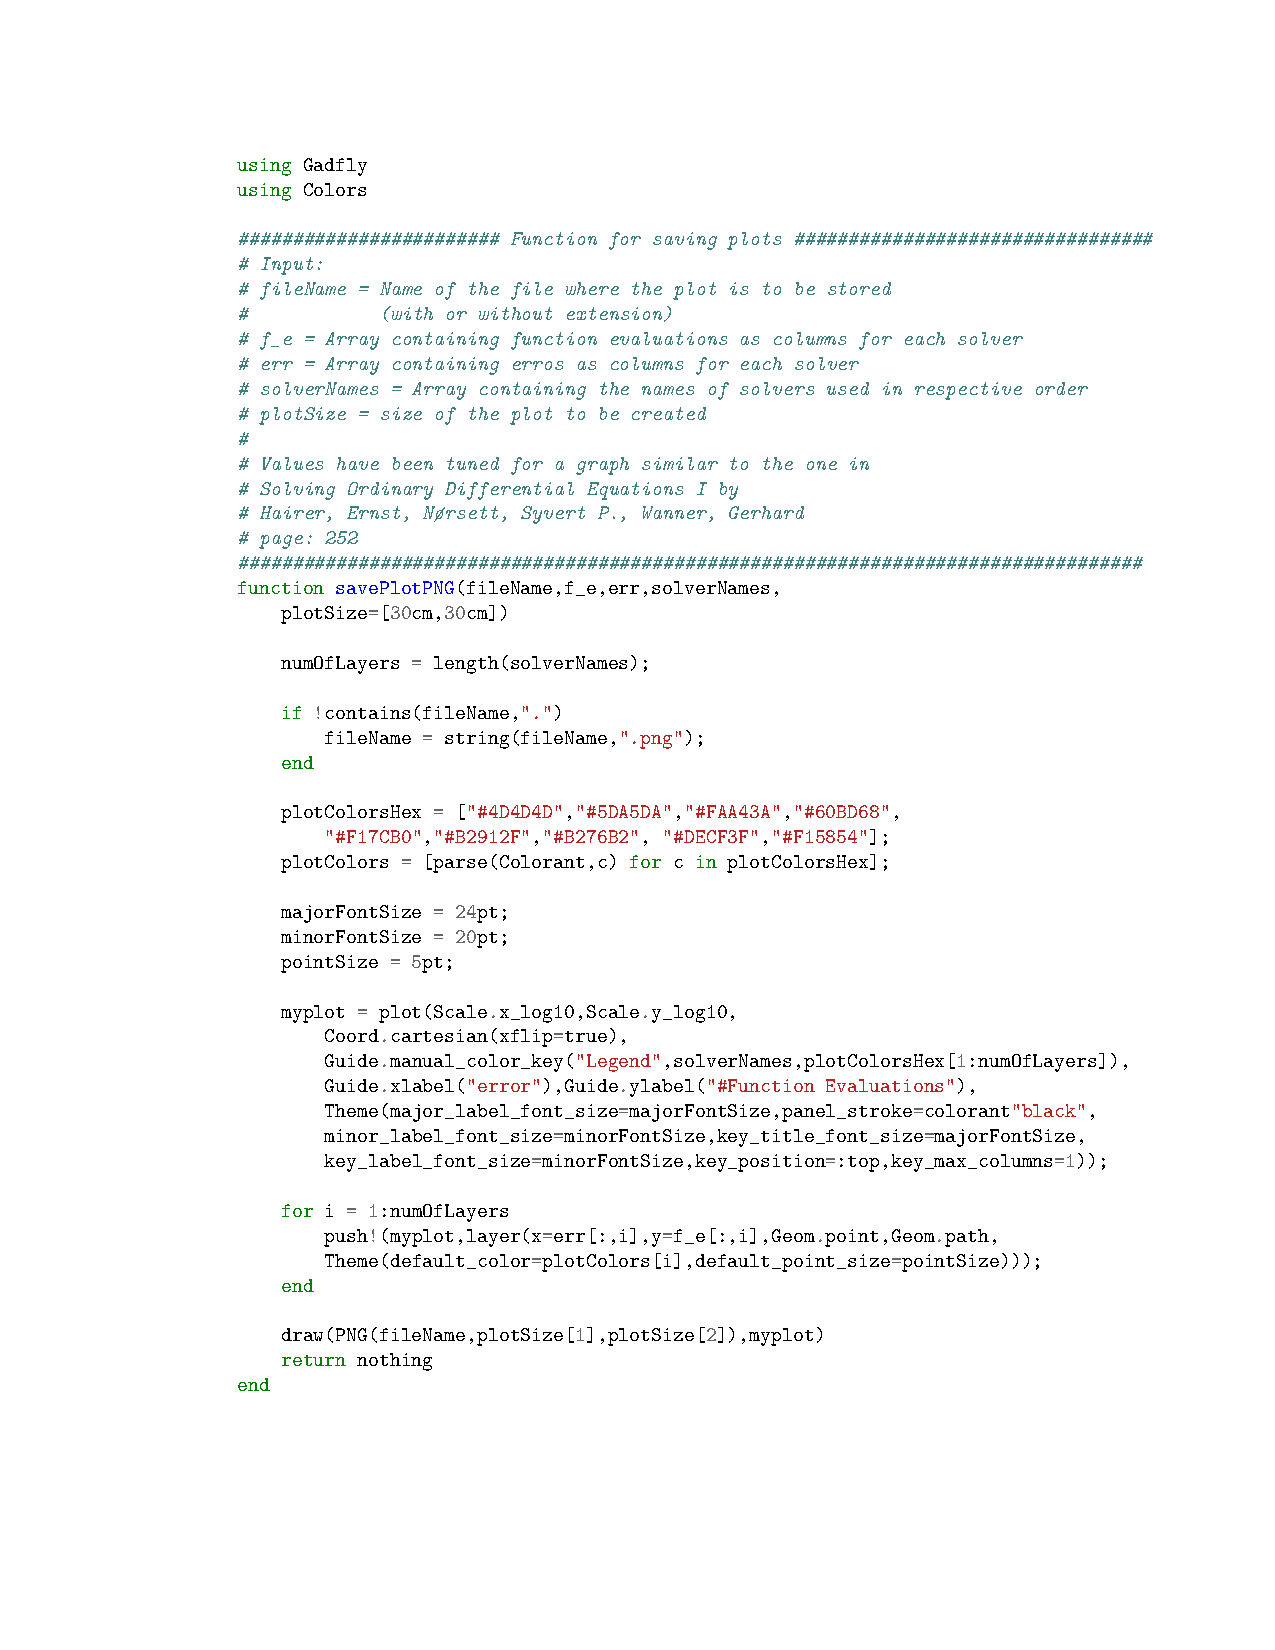
\includepdf[pages={1},pagecommand={\section{Appendix of Codes}
The codes over here are from March,2016. For updated codes refer \url{https://github.com/sonVishal/ODEInterface.jl/tree/master/myExamples/Codes}
\subsection{savePlotPNG}},scale=0.85]{../ImagesAndPDFs/Codes/code_savePlotPNG.pdf}

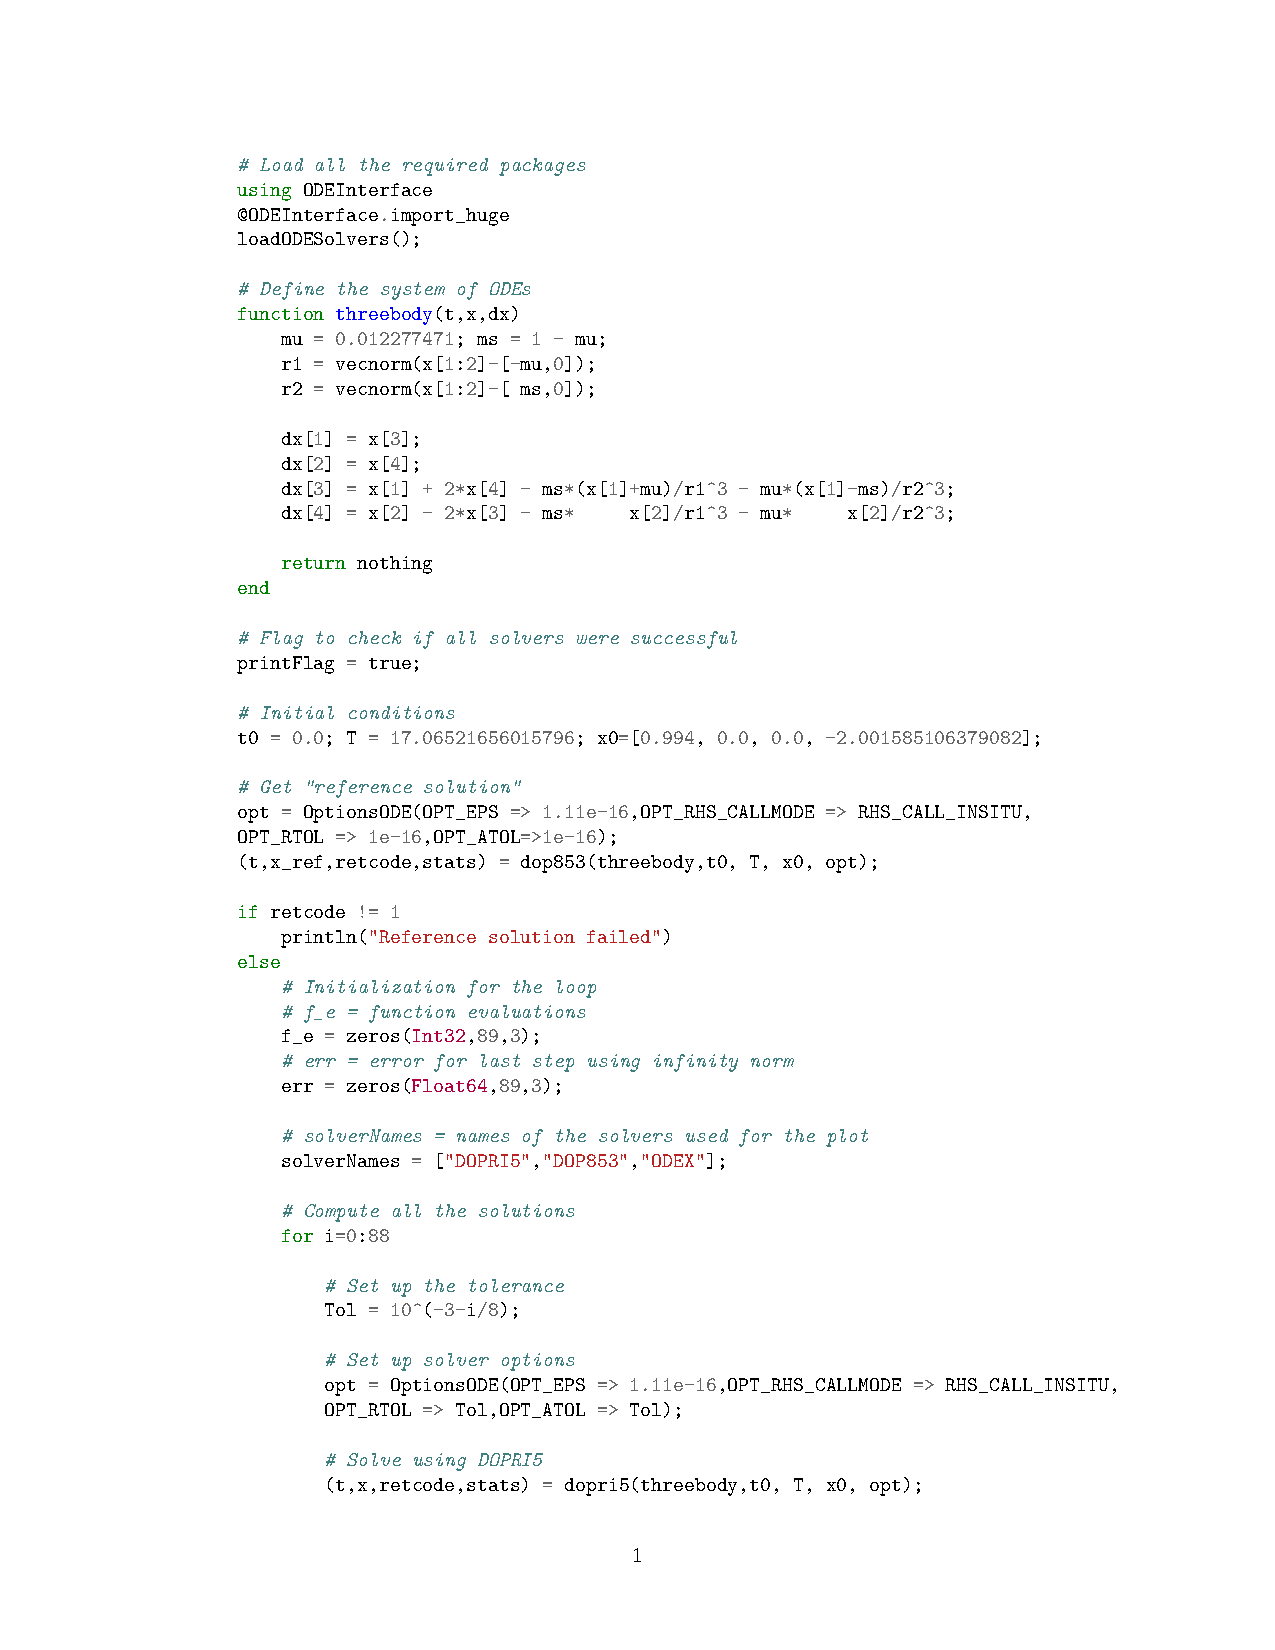
\includepdf[pages={1},pagecommand=\subsection{ArenPrecisionTest}]{../ImagesAndPDFs/Codes/code_ArenstorfPrecisionTest.pdf}
\includepdf[pages={2},pagecommand={}]{../ImagesAndPDFs/Codes/code_ArenstorfPrecisionTest.pdf}

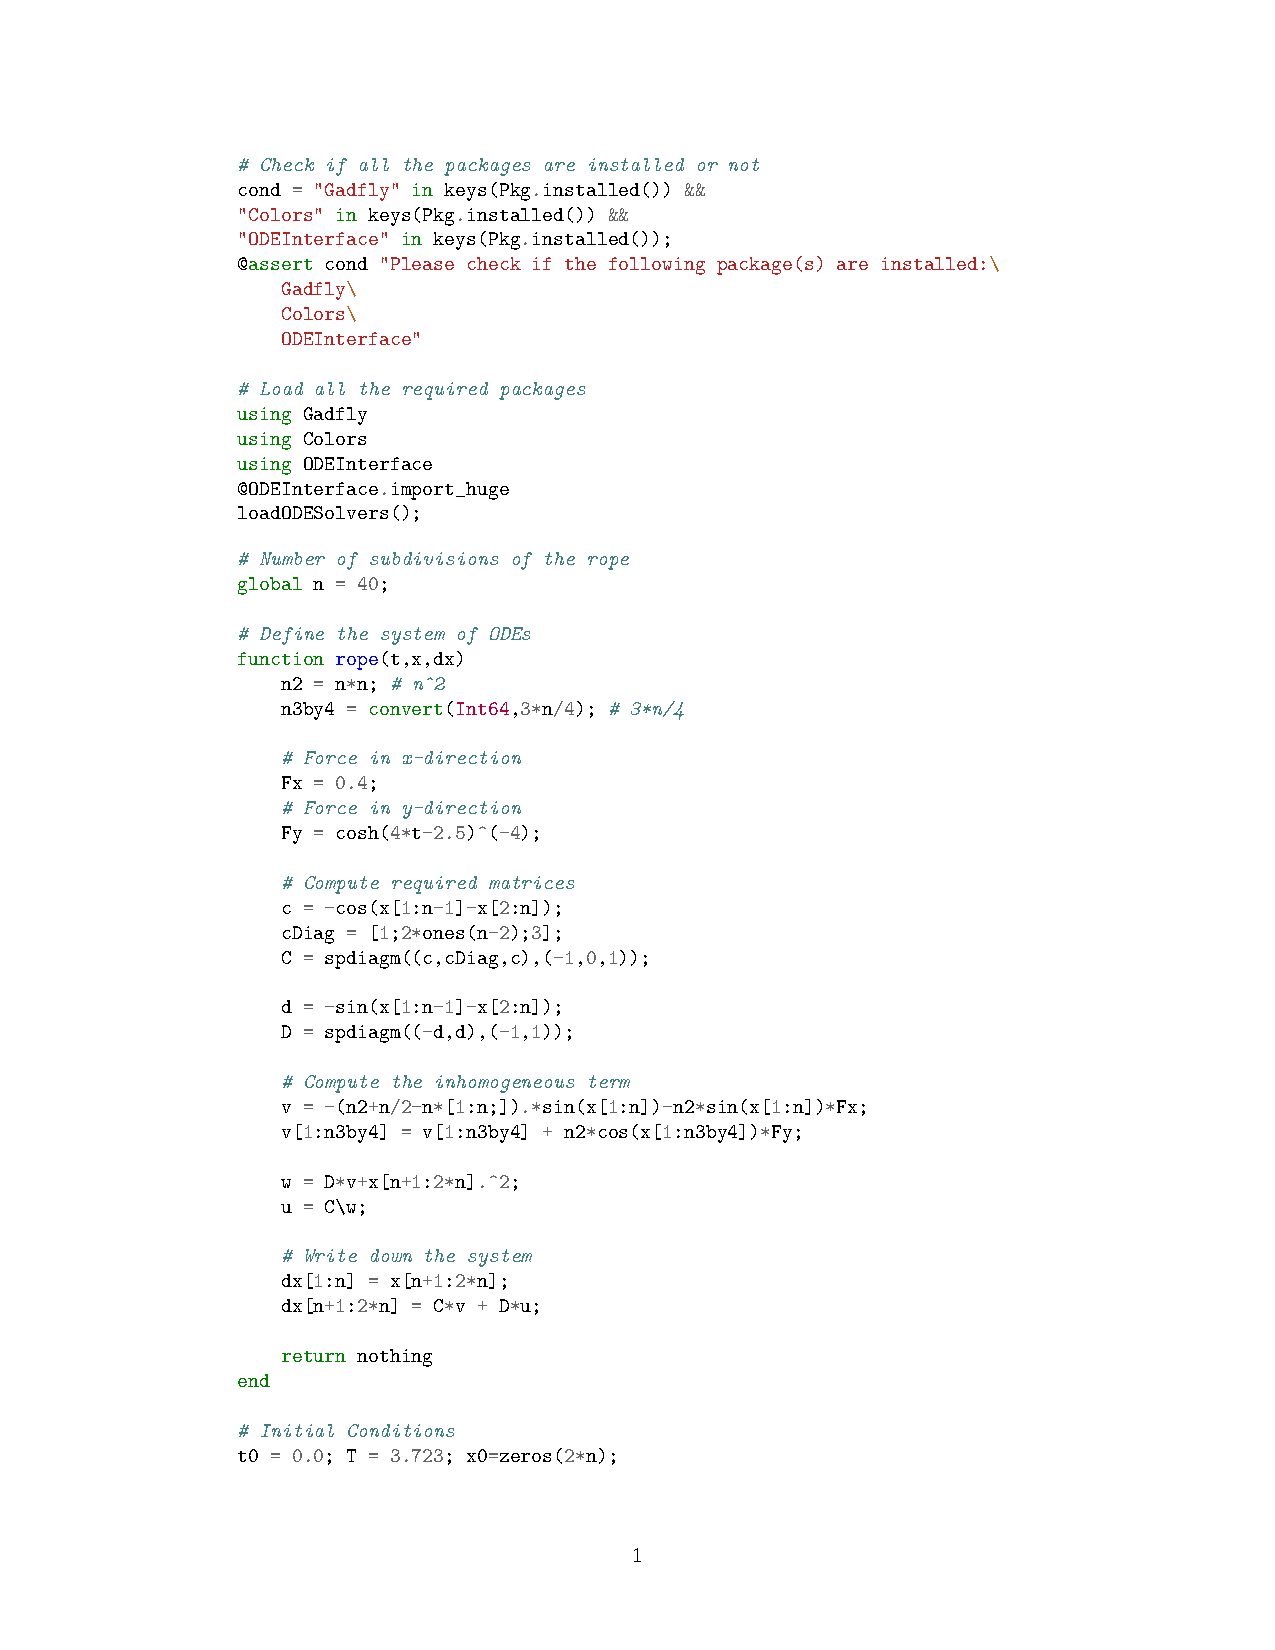
\includepdf[pages={1},pagecommand=\subsection{RopePrecisionTest}]{../ImagesAndPDFs/Codes/code_RopePrecisionTest.pdf}
\includepdf[pages={2},pagecommand={}]{../ImagesAndPDFs/Codes/code_RopePrecisionTest.pdf}
\includepdf[pages={3},pagecommand={}]{../ImagesAndPDFs/Codes/code_RopePrecisionTest.pdf}

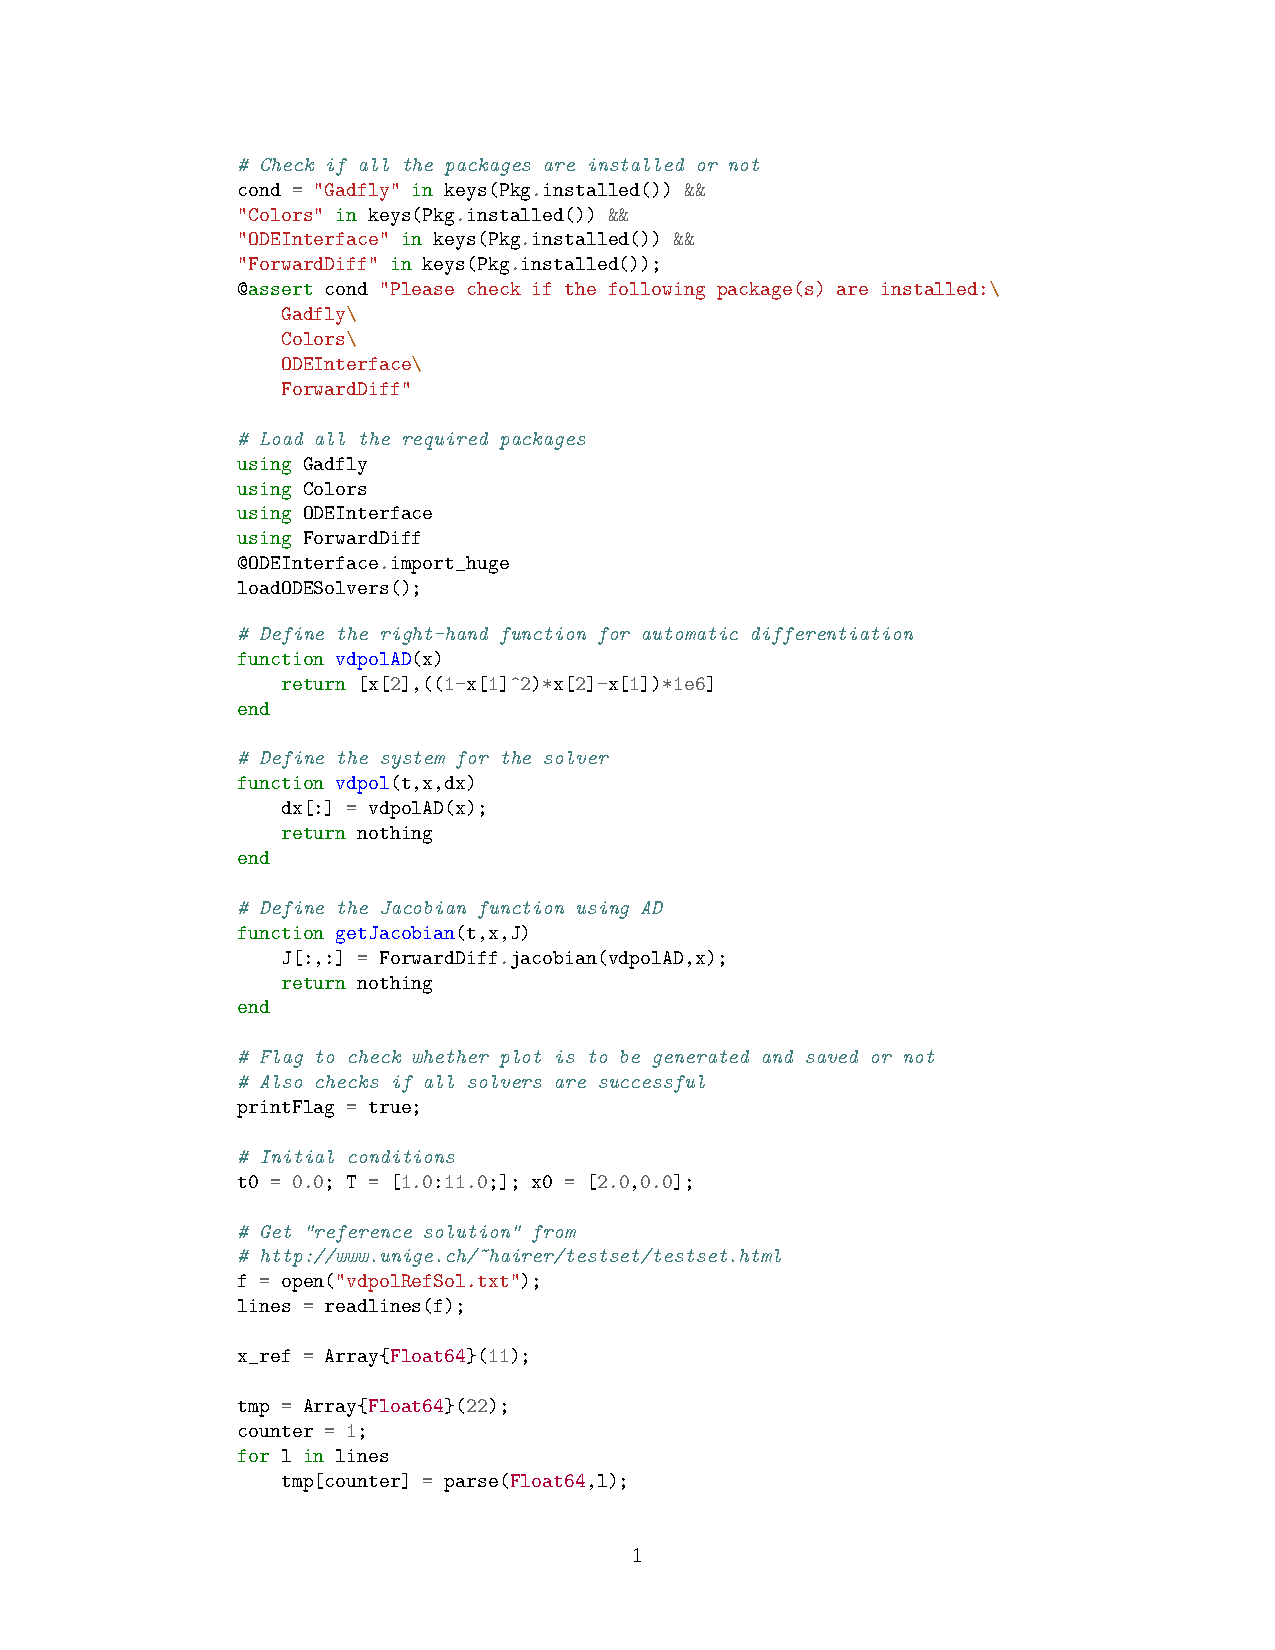
\includepdf[pages={1},pagecommand=\subsection{vdpolPrecisionTest}]{../ImagesAndPDFs/Codes/code_vdpolPrecisionTest.pdf}
\includepdf[pages={2},pagecommand={}]{../ImagesAndPDFs/Codes/code_vdpolPrecisionTest.pdf}
\includepdf[pages={3},pagecommand={}]{../ImagesAndPDFs/Codes/code_vdpolPrecisionTest.pdf}
\includepdf[pages={4},pagecommand={}]{../ImagesAndPDFs/Codes/code_vdpolPrecisionTest.pdf}

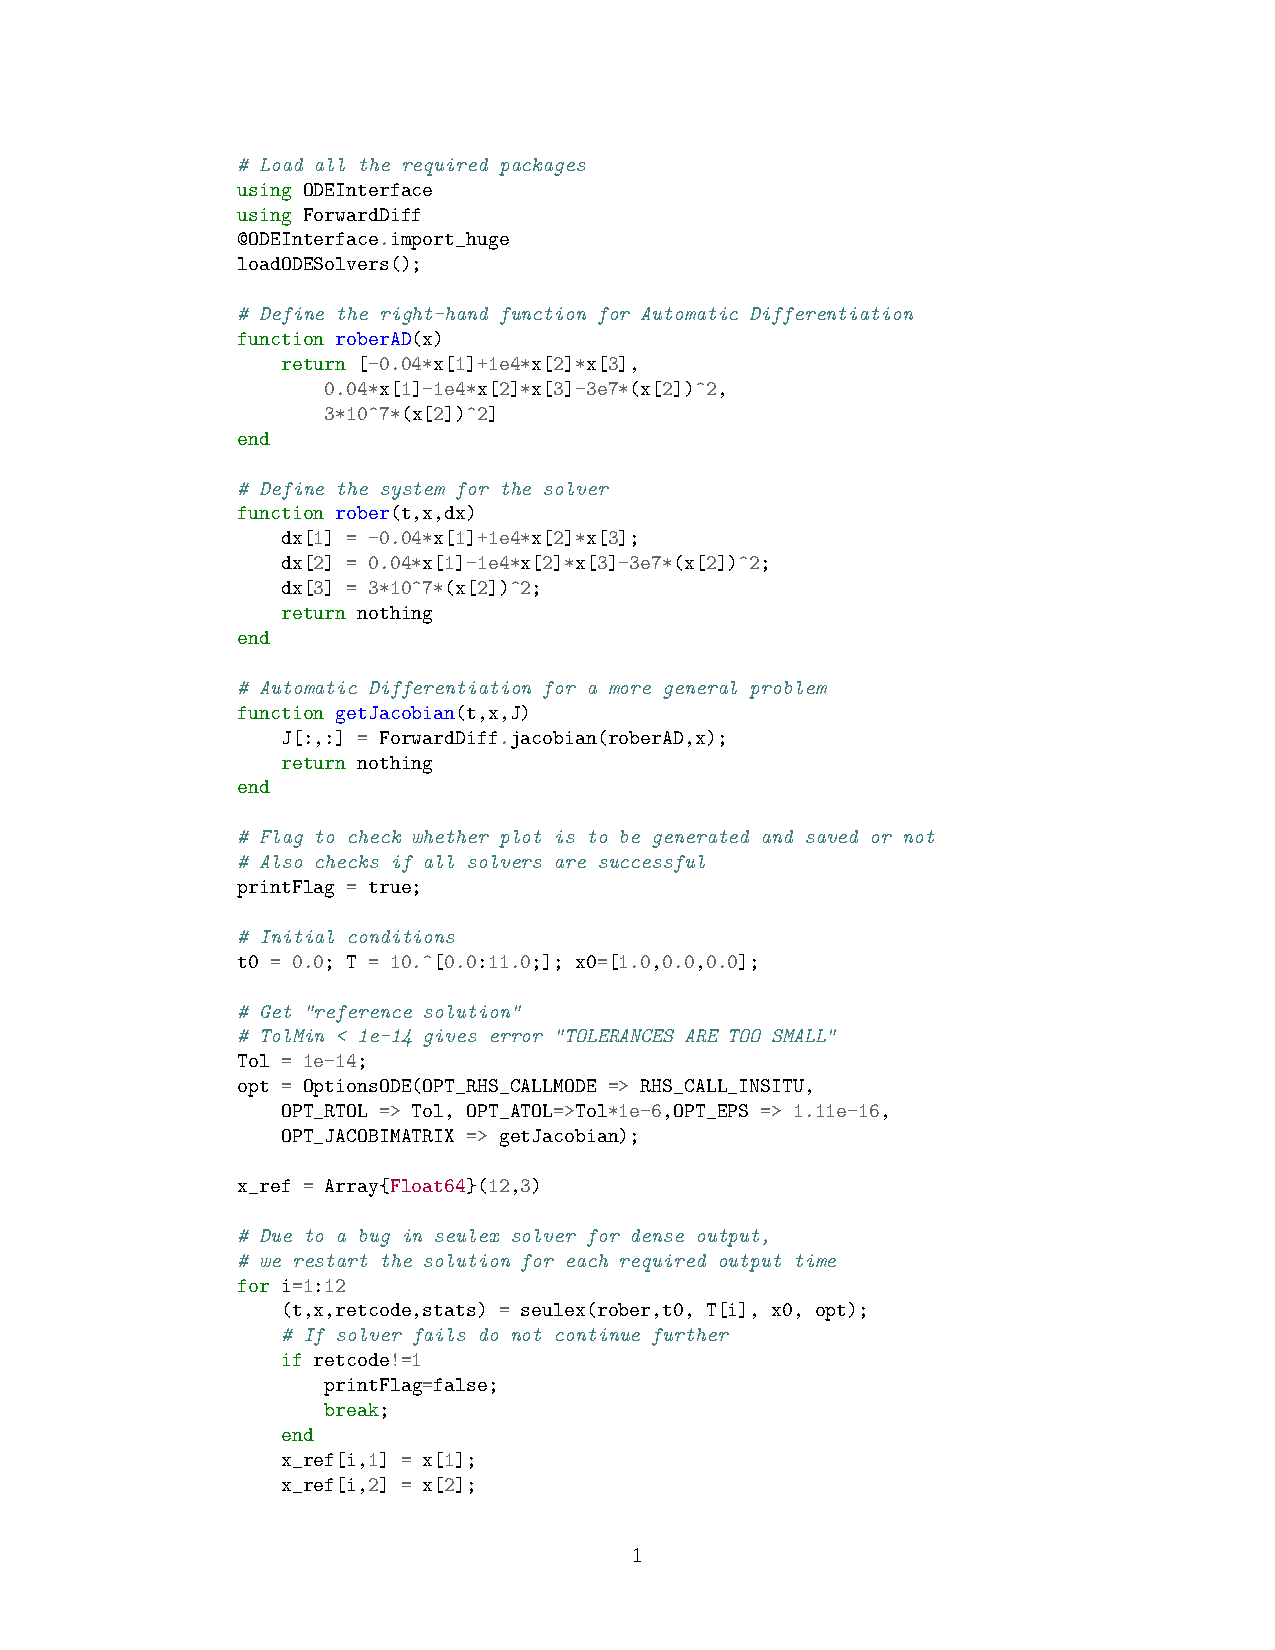
\includepdf[pages={1},pagecommand=\subsection{RoberPrecisionTest}]{../ImagesAndPDFs/Codes/code_RoberPrecisionTest.pdf}
\includepdf[pages={2},pagecommand={}]{../ImagesAndPDFs/Codes/code_RoberPrecisionTest.pdf}
\includepdf[pages={3},pagecommand={}]{../ImagesAndPDFs/Codes/code_RoberPrecisionTest.pdf}
\includepdf[pages={4},pagecommand={}]{../ImagesAndPDFs/Codes/code_RoberPrecisionTest.pdf}

\begin{thebibliography}{9}
\bibitem{nonStiff} 
Ernst Hairer, Syvert P. N\o{}rsett, Gerhard Wanner. 
\textit{Solving Ordinary Differential Equations I - Nonstiff Problems}. 
Springer-Verlag, Heidelberg, 1993.

\bibitem{stiff} 
Ernst Hairer, Gerhard Wanner. 
\textit{Solving Ordinary Differential Equations II - Stiff and Differential-Algebraic Problems}. 
Springer-Verlag, Heidelberg, 1996.

\bibitem{gadfly}
http://dcjones.github.io/Gadfly.jl/

\bibitem{ODEInt}
https://github.com/luchr/ODEInterface.jl/

\bibitem{ODE}
https://github.com/JuliaLang/ODE.jl

\bibitem{myODEInt}
https://github.com/sonVishal/ODEInterface.jl/

\bibitem{stiffRefSol}
http://www.unige.ch/~hairer/testset/testset.html

\end{thebibliography}

% section  (end)

\end{document}